% Created 2020-11-18 Wed 21:35
% Intended LaTeX compiler: pdflatex
\documentclass[11pt]{article}
\usepackage[utf8]{inputenc}
\usepackage[T1]{fontenc}
\usepackage{graphicx}
\usepackage{grffile}
\usepackage{longtable}
\usepackage{wrapfig}
\usepackage{rotating}
\usepackage[normalem]{ulem}
\usepackage{amsmath}
\usepackage{textcomp}
\usepackage{amssymb}
\usepackage{capt-of}
\usepackage{hyperref}
\author{adam}
\date{\today}
\title{Overview}
\hypersetup{
 pdfauthor={adam},
 pdftitle={Overview},
 pdfkeywords={},
 pdfsubject={},
 pdfcreator={Emacs 26.3 (Org mode 9.1.9)}, 
 pdflang={English}}
\begin{document}

\maketitle
\section*{Overview}
\label{sec:org7fe5846}

\subsection*{Course Structure}
\label{sec:org9d466ec}
This course is an introduction to media theory – a subcategory of
philosophy that emerged in the mid 20th century as an attempt to
understand the impact that new technologies were having on the
individual and, in a broader sense, society.
The general tone used to convey the ideas contained throughout the
notes and lectures will be an informal one, you refers to you the
reader, listener and student. We refers to the teachers, authors and
students that have been consulted in developing the material for this
course. Us refers to the group that we happen to find ourselves in at
any particular moment in time. And I refers to me, the teacher, Adam McCartney.
This course is intended to introduce undergraduate level music
students to the broader disciplines relevant for professional work in
the arts and humanities. There are those who would consider it absurd
that now, in the 21st century, investing in anything but a science
related degree is simply a waste. In the face of such beliefs, it is
worth pausing briefly to remember a simple point made by John Henry
Newman, that a solid education in the liberal arts equips a student
with tools that will ultimately lead them to become better engineers,
scientists, doctors, artists, lawyers and etc.


\subsection*{Philosophy of Teaching}
\label{sec:orgd2036f9}
\begin{center}
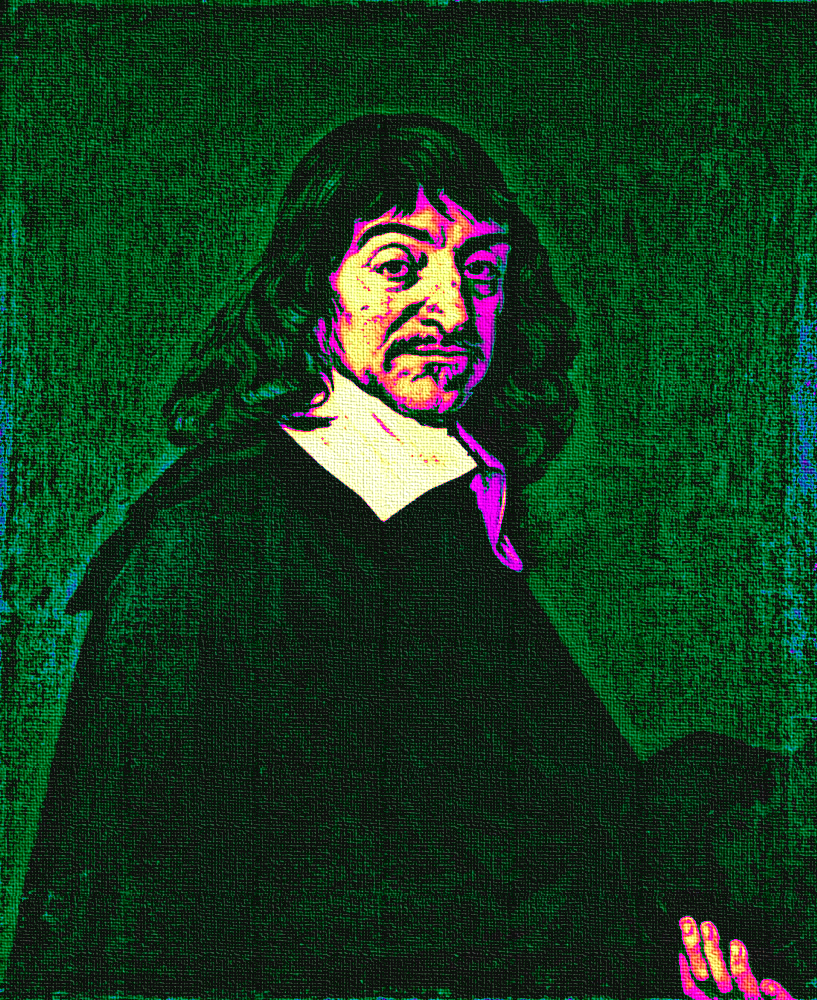
\includegraphics[width=.9\linewidth]{./descartes.png}
\end{center}
The satisfaction that can be gained through learning, teaching and
generally sharing information and can be immense. My more positive
experiences over the years as a student and teacher have tended to
come from courses, books, tutorials, videos, discussions that were
clear enough to allow enable an understanding of the topic from
first principles – that is to say that the material related to
the topic was assembled in such a way as to reveal its most
fundamental ideas. Its virtually always beneficial to ask rudimentary
questions about whatever it is that we are trying to understand, as
such questions will quickly reveal whether or not the topic under
discussion has a basis in fact.
This course also aims to introduce some of the core methods that are
useful anywhere that it becomes necessary to think about something:

\begin{itemize}
\item Discourse
\item Reason
\item Logic
\item Debate
\item Reference
\end{itemize}


\subsubsection*{7 Liberal Arts of the medieval university}
\label{sec:org2ced3e4}
\begin{itemize}
\item Grammar
\item Rhetoric
\item Logic
\item Geometry
\item Arithmetic
\item Music
\item Astronomy
\end{itemize}

\subsection*{Where and how to access material}
\label{sec:org564d4da}
The primary source of information for topics presented in this course
can be found in the VMI digital library, which is labelled \emph{Academic
Resources For Students} and will appear as a link on the homepage of
your Moodle eLearning profile.
Please take the time to do the readings, this will prepare you for the
discussions that will take place during class. Thinking about things
is a practical exercise, it‘s the same as riding a bicycle or learning
to play an instrument. That means that the only way that you are going
to learn how to think is by engaging with the readings and
exercises. Much the same as any activity that is worth learning,
thinking is difficult and takes a lot of patience to get right.
The texts that were chosen to be part of the course are all written in
an accessible style and are not overtly academic or
technical. Nevertheless, they do contain  ideas and arguments that you
might not get on the first reading.  My two favorite reading
disciplines  from when I was an undergraduate were the practice of
reading for a pre-allocated amount of time and also reading each text
at least three times in preparation for a class.

\subsection*{Portability and how to apply course content}
\label{sec:org223ecb5}
Should you try and tell your piano tuner about Ludwig Wittgenstein‘s
ideas on the formation of knowledge? Definitely not! In fact, they
would be more likely to charge you extra fees just to get your piano
tuned if you chose to do so.
So where exactly can this knowledge be applied? A friend of mine is a
hobby programmer and he recently told me his principle approach to
work. He called it „eat your own dogfood“. Now obviously the idea of
eating any kind of dogfood does not sound particularly appetizing, but
it is worth considering that dogs can also eat cake. The simple idea
here is that whatever type of idea or discipline you develop, it is
better first practiced on yourself before inflicting it upon the rest
of us; when properly cultivated a discipline is a way to nourish,
develop and sustain.




\section*{The long 19th century (1789 - 1914)}
\label{sec:orge26237e}

\subsubsection*{A brief history of art leading up to the industrial revolution}
\label{sec:orgdda547b}
The renaissance had shown that the rise of merchant classes was
possible, and that there was room for a talented craftspeople to build
a career out of a good reputation. Still, even the most talented
artists from the renaissance and baroque periods were subjects of
some royal court and often patronized (though less commonly so than in
the middle ages and early renaissance) by the clergy. The dominant
motives of these eras were, for instance, dedicated to the nobility
and to the church. An appreciation for human ingenuity was growing and
quietly, a new philosophy of reason and enlightenment was being born.


\subsubsection*{Art in the Age of Revolution (1789 - 1848)}
\label{sec:orgb3202ae}

Before it turned into a bloody mess, the core ideals of the French
Revolution (freedom, equality and brotherhood) seemed to be an
articulation of the broader hopes of humanity for a brighter future.
Many of the artists of the late 18th and early 19th centuries echoed
these newly formed ideas of the enlightenment.

\begin{itemize}
\item 50 years that included late Mozart, Haydn, Beethoven, Schubert, Goethe, Dickens,
Dostoevsky, Verdi, Wagner, Mary Wollstonecraft, Mary Shelly
\item Art made to appeal to a literate public that was increasing in
size
\item The invention of machinery reduced the cost of physical labor for
many, meaning there was more free time for education and pastimes
\item Aesthetic themes often contained pastoral elements, or sought to
simplify harmonies and form.
\item The influence from classical antiquity frequently appear, along with
references to similar threads from the renaissance
\end{itemize}

\begin{figure}[htbp]
\centering
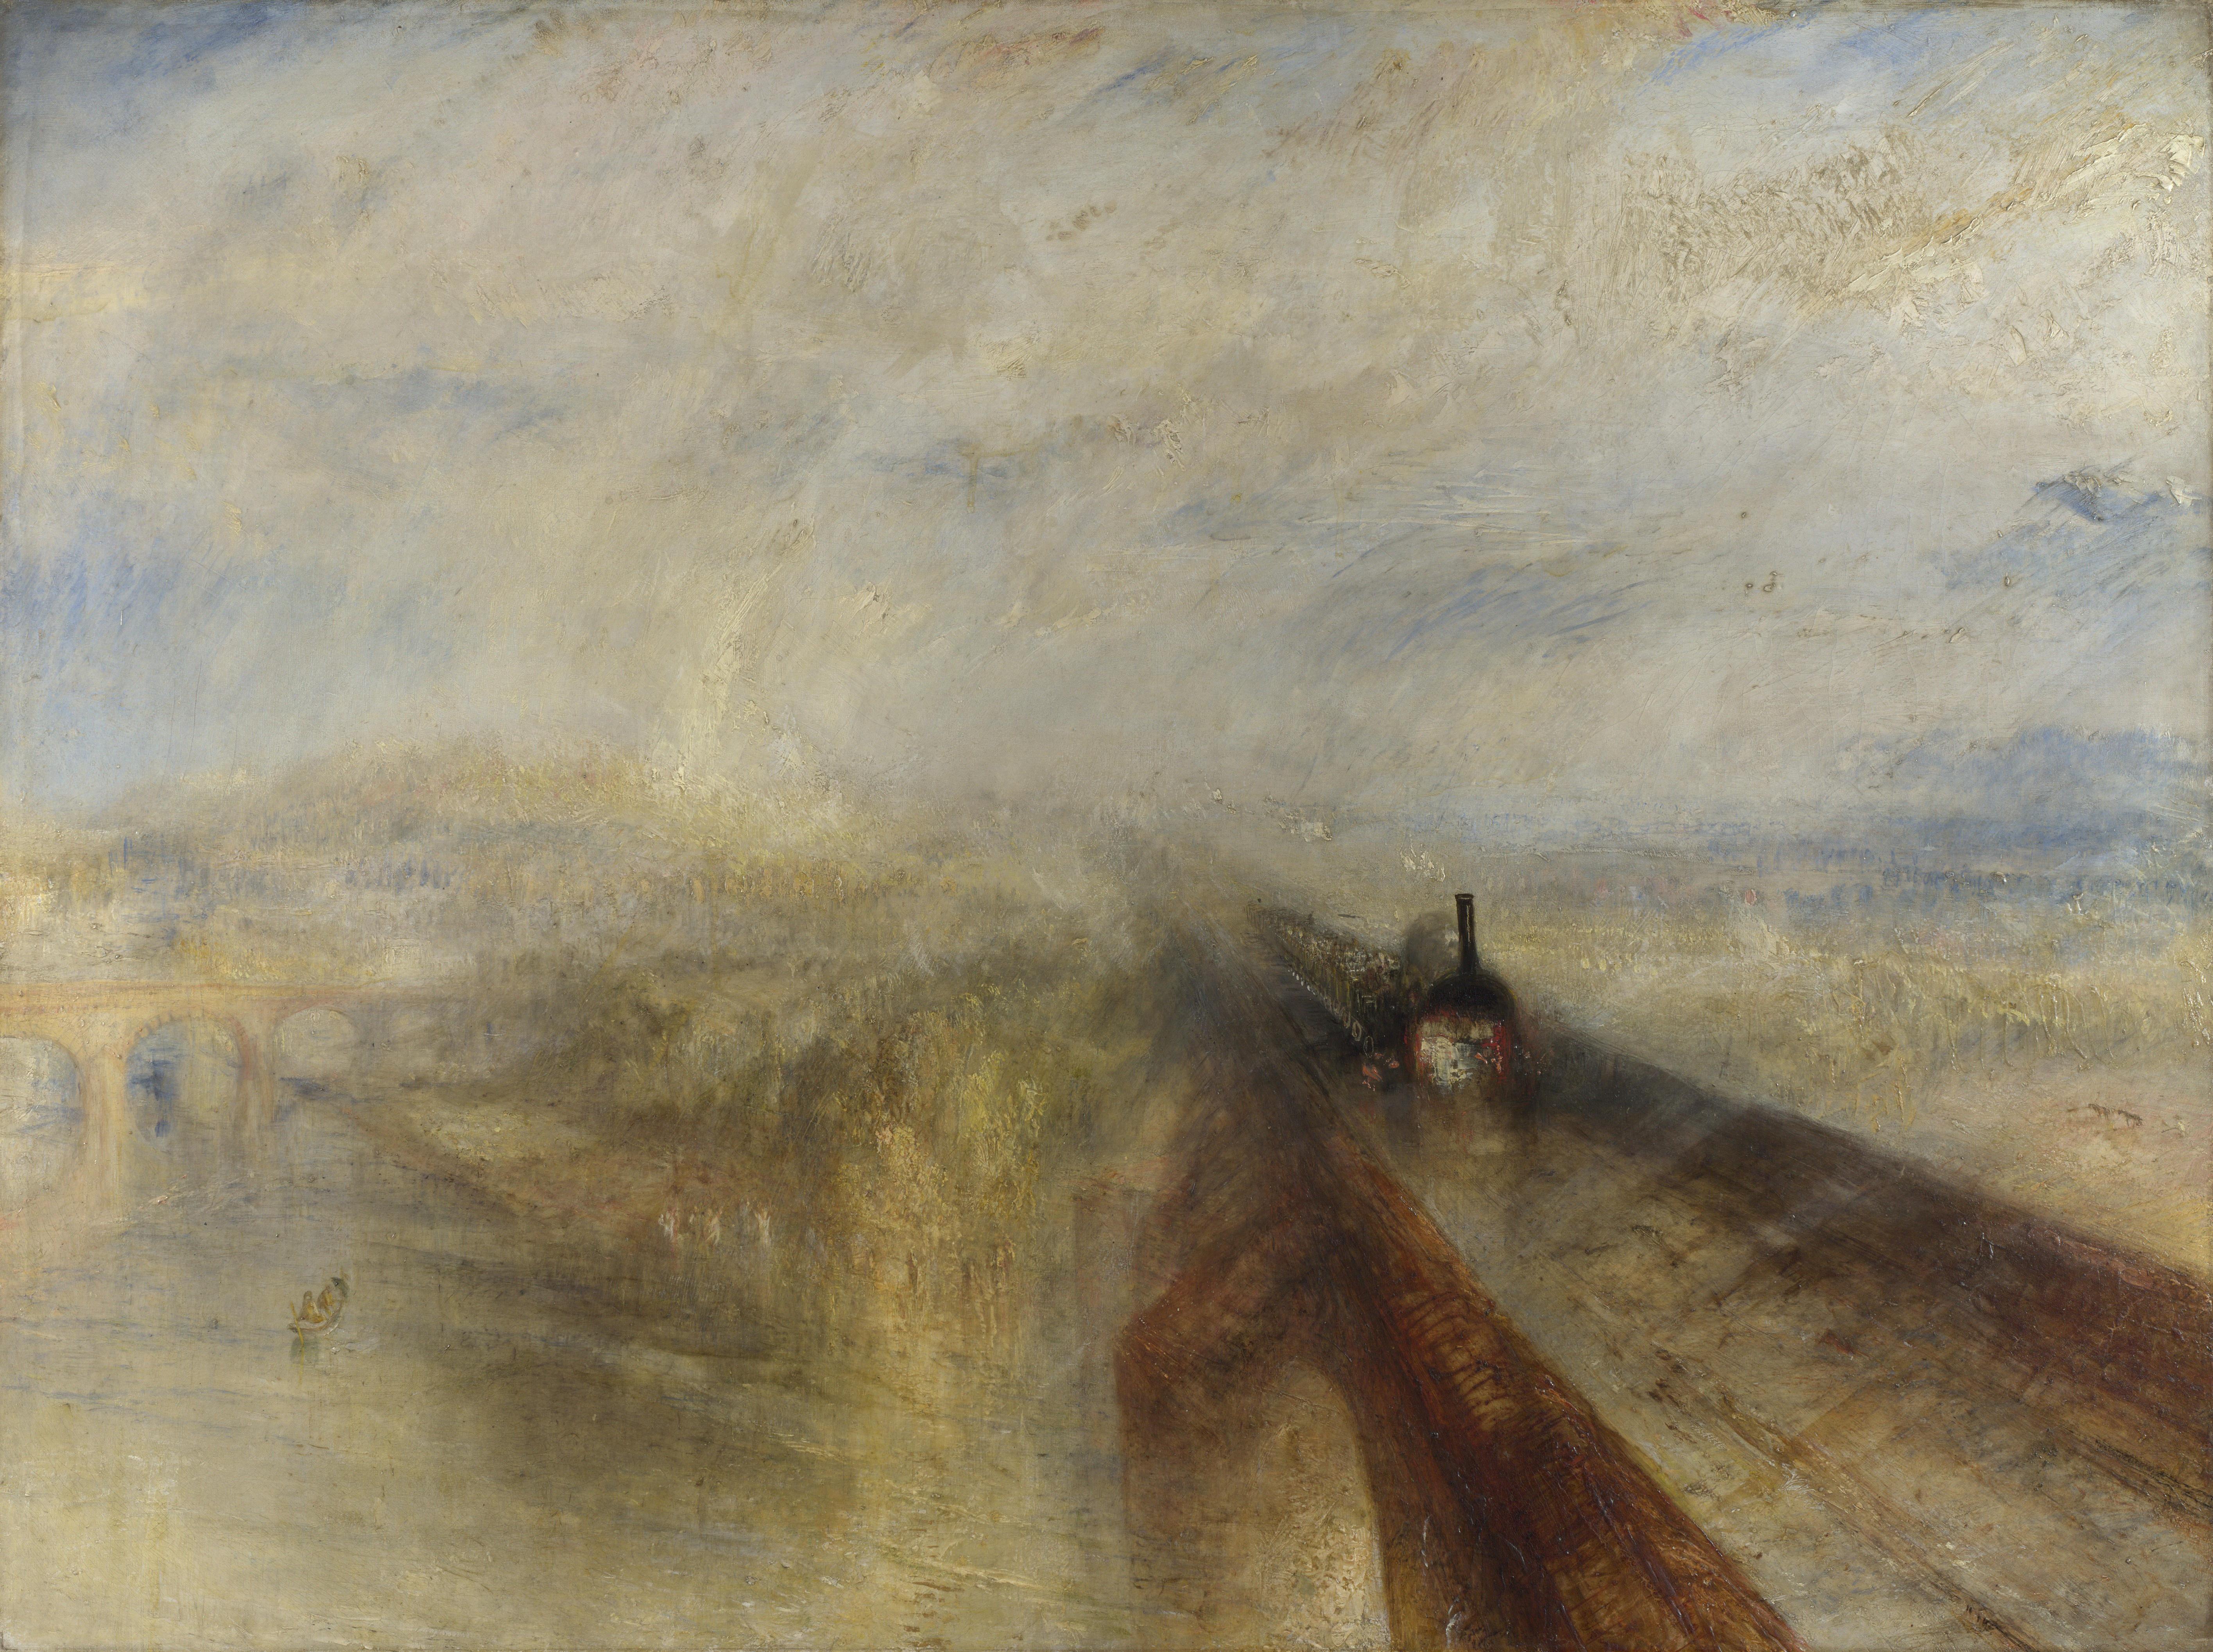
\includegraphics[width=.9\linewidth]{./Turner_-_Rain,_Steam_and_Speed_-_National_Gallery_file.jpg}
\caption{William Turner - Rain, Steam and Speed}
\end{figure}

\subsubsection*{Utopia}
\label{sec:orgeabc77f}

Much of the art of the age focused Utopian ideals, be they either in
some possible future or some glorified past: there were large
collections of folk tales, songs and verses that emerged during this
period that bore testament to the vision of "the folk" as being
inherently virtuous. The new movements toward industrialized living
and a faster pace of life, on the other hand, was often viewed with at
least the usual amount of suspicion. Of course, the of a fall from
grace and the quest for redemption is literally as old as Adam and Eve.

\subsubsection*{Art in the Age of Capital (1848 - 1875)}
\label{sec:org1e8b620}

Having seen what the first half of the 19th century delivered in terms
of the arts, it's not surprising that this period during the later half of
the century appears somewhat underwhelming. Perhaps the real
achievements.
\begin{itemize}
\item the era produced a rather curious architectural style with
increasingly large proportions - this marks a contrast to the
classically influences in the styles (like Biedermeier) that
immediately preceded, where in central focus were human proportions
\item funding structures of the arts changed: they were now supported by
governments, bourgeoisie and increasingly the emerging working /
middle class
\item the Viennese ring serves as a good example to the monuments of the age
\item first appearance of technically reproducible works of art (early
photo camera had an immediate and profound effect on painting
\item arts were in every sense popular by the third quarter of the
century, with widely distributed novels
\item possible for artists to earn a good living and many (even if not
rich) were well respected
\item arts came to occupy a semi-religious position for many of the new
middle class, also (in the case of the German speaking world) a
symbol of success and status to rival Britain's economic spoils
\item the artists were seen as sources of truth, authorities on beauty
\end{itemize}



\subsubsection*{Art in the Age of Empire (1875 - 1914)}
\label{sec:org113162b}
Bourgeois identity crisis
\begin{itemize}
\item Orientalism
\item pastiche
\end{itemize}

Established and entitled artistic circles
\begin{itemize}
\item the Successions of Vienna \& Berlin
\item the New English Arts Club
\item successors to the French Impressionist Exhibition
\end{itemize}

The emergence of the avaunt-grade
\begin{itemize}
\item very limited public reception
\item the anti-reality star? (like Picasso, appreciated for their
phenomenal output as opposed to the qualities or content of the work)
\end{itemize}

The birth of cinema


\subsection*{The short 20Th century (1914 - 1996): Art in the Age of Extremes}
\label{sec:orgd6ab149}
\subsubsection*{Features of the early 20th century art landscape}
\label{sec:orgacf4f13}

\begin{itemize}
\item Modernism
\item Dadaism, Constructivism, Surrealism
\item Decided move away from conventional Bourgeois tastes
\item Europe (Paris) between the wars
\item The invention of cinema \& jazz
\item Battleship Potemkin \{ watch?v=VMWMq4AEyjU \}
\item Jazz: syncopated Afro rhythms meets mechanical reproduction
\item Murillo was out El Greco was in
\item Also rejected: Age of Capital and Age of Empire
\item Viennese Ring considered pompous \& inauthentic
\item most of the avant garde artists identified with progressive politics
\item rise of Hitler and Stalin meant that most of the avant garde immigrated to the USA
\item James Joyce Ulysses: going to the common man
\item Mass media and propaganda
\end{itemize}

\subsubsection*{Postwar Arts}
\label{sec:orge206b45}

\begin{itemize}
\item Rock \& Roll, the LP
\item the advertising industry
\item the emergence of pop art
\item Shift away from Europe
\item The establishment new social democratic norms post 1950 - massive increase government funding for the arts tax-breaks in the States for wealthy patrons
\item Art as Investment
\item Massive Expansion of higher education
\item Classical music - decline in old genres concealed by the enormous increase in their performance mostly a repertoire of dead classics
\item Personal Electronics
\end{itemize}


\section*{Aesthetic and sociological perspectives}
\label{sec:org738a5b8}
\subsection*{Critical Theory}
\label{sec:orge1498dc}

Reference: \url{https://plato.stanford.edu/entries/critical-theory/}

In the narrow sense, critical theory refers to a strain of Marxist
philosophy that appeared in early 20th century Germany. It is critical
in the sense that it seeks human "emancipation from slavery", acts as
a "liberating \ldots{} influence", and works to "create a world which
satisfies the needs and powers" of human beings (Horkheimer 1972, 246)

Key figures of "the Frankfurt School": Max Horkheimer, Theodor Adorno,
Marcuse, Benjamin

Being a strain of Marxist philosophy, central to critical theory is a
critique of Capitalism. Furthermore, a strong emphasis is placed on a
belief that civil society and human culture in general is undergoing a
process of degeneration due to the commodification of artistic
production and aesthetic experience.

It could be argued that much of critical theory is based on a
revivification of an aspect of Kant's categorical imperative: namely,
that one should avoid using people (including oneself) as a means to
an end. A critical theorist such as Adorno might argue that
contemporary pop that has been used in the service of some form of
advertising, is ultimately less moral and therefor less good or
effective than say, Beethoven's 7th symphony. (Adorno \emph{really} liked
Beethoven and was big into the idea of "absolute" music).

By the same reasoning, one could argue that the whole discipline of
Critical Theory is morally corrupt due to the simple fact that it
essentially seeks to hi-jack and politicize branches of philosophy
such as aesthetics (which are by no means inherently political).

\subsubsection*{Walter Benjamin}
\label{sec:org8b56c8a}
A Berlin born art theorist / philosopher whose writings were a large
influence on Theodor Adorno. Also a fairly dedicated Marxist, who

\subsubsection*{The Work of Art in the Age of Mechanical Reproduction}
\label{sec:org2ee32e9}

\subsection*{John Dewey's Aesthetics}
\label{sec:org23ba29f}
\subsubsection*{Pragmatism}
\label{sec:org57afa0d}
Originated in the United States towards the end of the 19th century,
largely as a reaction to what was considered the overly theoretical
and technical nature of continental philosophy.

Notable Figures included William James and George Herbert Mead, who
had the idea that it was only possible to define a person through
their actions in the world.

\subsubsection*{The Live Creature}
\label{sec:orga8d1ea1}

Notes on reading: \url{https://plato.stanford.edu/entries/dewey-aesthetics/}

First couple of points to note relate to the historical evolution of
aesthetics. With the rise of nationalism and imperialism, art became
disassociated from religious right and with the growing dominance of
capitalism, became more about documenting material wealth than
integrating personal with collective experience.

This idea of the quality of experience is seemingly central to Dewey's
aesthetics. It follows quite logically that experience happens
essentially in conjunction with the environment and not just \emph{in}
it. Whether or not life experience can be reduced solely to the basis
of needs and conquest, is not so clear. I do not think that it is self
evident that all conflict and resolution arises from the frustration
or gratification of basic physical or physio-psychological urges.

Nevertheless, it is possible to imagine how Dewey might try to
structure his thought at this stage as he suggests that harmony and
equilibrium arise from the resolution of tension. Awareness of this
process, the rhythmic alteration between states of unity and disunity
signifies conscious participation in the phenomenon of experience.

Dewey seems to suggest here that emotions are breaks in experience,
something to be understood in retrospect. More specifically he refers
to emotions as signifiers that disrupt experience. This does make some
sense, as the presence of an emotion seems, quite certainly, to
require a level of abstraction that seems to move the subject into an
acute awareness of the distinct mode, through which he now views experience.

He sets up an interesting comparison between scientist and artist,
shows that both are trying to shape material according to their thought processes.

He points out that nature already has emotional qualities. That some
aspects may appear comforting or disturbing.

Aesthetic experience then involves a temporal process where action,
feeling and meaning are one.  The cumulative effect of these on one
another is balance. This is only possible, in a dynamic world, where
experience takes place.

Passing out of disturbance into harmony can provide man's most intense
experience. Happiness is the result of a deep fulfillment in which our
whole being has adjusted to the environment. This seems to directly
contradict what he says above about emotion, although on a more subtle
level he seems to be suggesting something closer to integration here
than happiness. Personally, I would place the core of aesthetics at integration.

\subsubsection*{Emotions}
\label{sec:orgd385141}

The previous section suggests that aesthetics is essentially an act of
integration. The experience of this act, ultimately leads to an
emotional experience. Emotions are not static, they posses dynamic
qualities and can grow or shrink over time.







\section*{Media Theory}
\label{sec:org8aecbfb}
\subsection*{Marshall McLuhan}
\label{sec:orgcd0a5f4}
\subsubsection*{Biographical Note}
\label{sec:orgcc8cf35}
\begin{itemize}
\item born Edmonton, Canada 1911
\item died 1980
\item BA/MA at the University of Manitoba
\item Doctoral Studies at Cambridge
\end{itemize}
\url{https://www.marshallmcluhan.com/biography/}


\subsubsection*{Early Influence}
\label{sec:orgff79302}
At Cambridge (entering in 1934) he studied under the professors I.A. Richards and
F.R. Leavis.

It's worth considering that there were some pretty incredible advances
taking place in the fields of Mathematics and Physics (both
theoretical and applied) during the first half of the 20th century.

\begin{itemize}
\item Bertrand Russell and Alfred North Whitehead had published "Principia
Mathematica", both of whom held professorships in mathematics at Cambridge
\item Ludwig Wittgenstein started a fellowship at the University in 1929
\item Alan Turing studied there as an undergrad from 1931 to 1934 and was
elected a fellow of King's College in 1935 (at age 22) after his
dissertation offering a proof of central limit theorem was well
received
\end{itemize}

Besides the obvious name dropping, the purpose of pointing out these
figures is to emphasize that there was a lot of "technical" academic
work happening at Cambridge during this time. In particular, Russell \&
Whiteheads work on finding a formal description of mathematics saw the
development of specialist notation.

In an attempt to keep up with these advances, fields more
traditionally rooted in the humanities, themselves began to embody the
new practices of logic and formalism as they emerged from mathematics,
physics and early computational theory.

It seems that I.A. Richards was particularly interested in forming a
new, multidisciplinary approach to literary criticism that could give
formalist, self-contained and objective accounts of what was being
said in any literary work. It appears that to some degree, Richards
was trying to incorporate cybernetics into his theories on literary
criticism.

Thinking about the human mind as one part of a cybernetic system, was
an idea that influenced McLuhan profoundly, and research in and around
this idea became a central part of his work throughout the rest of his
career.

\subsubsection*{The book as technology}
\label{sec:orga097d9b}

\emph{"Water is unknown to a fish until it discovers air"}

In "The Gutenberg Galaxy" McLuhan presents a dazzling array of ideas,
that often closely focus on the multi-sensory (or multi-dimensional)
context of literary ideas. For instance, he writes about Shakespeare's
use of perspective in King Lear, pointing out that it may be the first
time that a writer has employed the use of a three-dimensional first
person perspective on a scene within the context of a literary
work. For McLuhan, the interesting point here is that the written word
seems to been reaching out beyond the page, and evoking our other
senses to aid our perception of the scene.

Print is an extension of writing, which itself is an extension of
speaking and in turn thinking. The process is inherently circular,
a new technology emerges to form a super set of the technology that
immediately preceded it.

For McLuhan, technology is always an extension of the mind (the
cognitive/sensory apparatus) and therefor it influences the formation
of ideas.


\subsubsection*{The Medium is the message}
\label{sec:orgb6b8ac6}
\url{https://web.mit.edu/allanmc/www/mcluhan.mediummessage.pdf}

\begin{itemize}
\item The nature of human relationships, interaction and work was shaped
by the first industrial revolution: the introduction of the machine
and the philosophy of the "division of labor"
\begin{itemize}
\item The essence of the electronic/digital revolution is entirely the
opposite of this because (integral \& decentralised)
\end{itemize}

\item First principles look at the nature of certain types of business in
the (post)-industrialized world
\begin{itemize}
\item IBM \(\rightarrow\) information processing
\item AT\&T \(\rightarrow\) moving information
\end{itemize}

\item Does technology add itself on to what we already are?

\item What does it mean to understanding the "grammar" of a particular technology?

\item How are artists in a unique position to encounter technology?

\item The fact that it is currently being debated as to whether big tech
should be treated as utilities is reminiscent of the idea that
technological media are resources comparable to water, coal, cotton
and oil.

\item Bertrand Russell: the technique of the suspended judgement was the
great discovery of the twentieth century

\item A.N. Whitehead said that of the 19th century it was the discovery of
the technique of discovery (starting with a result and working
backwards)

\item The work of the artist represents the only documentation of the
continuous adjustment to the various new factors of personal and
social life as they are extended.

\item The artists job is to engage with the present totally
\end{itemize}


\section*{Computing: Another historical interlude}
\label{sec:orge5d1f2c}

"Give me six hours to chop down a tree and I will spend the first four sharpening the ax"
\begin{itemize}
\item Abraham Lincoln
\end{itemize}

The next couple of sections serve to offer a very brief overview of the history of computing. Although computers are ubiquitous and a thorough discussion of the history of their development might be of more interest to those with a more technical interest, the culture around computing is actually pretty interesting. We've been talking a lot over the past couple of lectures about some of the sociological developments that have taken place over the past 150-200 years. We've focused on the artist and the means of production used to make art. Also, we've asked some fairly general questions about how the context within which art is made (or taught) influences the production. The purpose of this rather long-winded exposition is to spend some time reasoning about our current environment. The better that we are able to perceive the situation, the more likely it is we will reach for the right tool when it comes time to do the work.

\subsection*{What the hell is a Unix?}
\label{sec:orgbd4fb46}

Unix is a simple operating system that was born in 1969, invented by Ken Thompson at Bell Laboratories (a research branch of AT\&T). This is not really the place to go into a detailed history of how it developed, if you are interested, check out Brian Kernighan's writings on the subject, along with Eric S. Raymond and Mike Loukides. All will offer a slightly different perspective on the origins of Unix and how it has developed over the years.

There are some diverging opinions on why Unix has been successful as an operating system. It's not uncommon to hear people speaking in hushed tones about free software and the open source movement as reasons for its longevity and success. Others will put it down to factors associated with the nature of the computer hardware business in the 1980s. Either case is not particularly important to understand for our purposes. What is important is that there seems to be some consensus around how its use in Universities and research environments ultimately contributed to its popularity. The point here being, that the University is still one of the rare places where a more open-ended form of creativity is encouraged. Unix suits researchers because it is accessible, easy to use and fun to hack.

\subsection*{History of the internet}
\label{sec:orgc4d5556}
\begin{itemize}
\item invented as a way for mutually trusting and cooperative parties to exchange information
\item for a more detailed history see \ldots{} the internet
\end{itemize}
\subsection*{Internet overview}
\label{sec:orgd1e1e88}

\subsubsection*{Devices}
\label{sec:org4f6e596}
\begin{itemize}
\item host = end system, runs apps
\end{itemize}

\subsubsection*{Communication Links}
\label{sec:orgf50f0f4}
\begin{itemize}
\item fiber, copper, radio, satellite
\end{itemize}

\subsubsection*{Packet switches}
\label{sec:orgc53837f}
\begin{itemize}
\item routers and switches
\end{itemize}

\subsection*{Service view of the internet}
\label{sec:org3c3ab40}

\subsubsection*{Provider of services to apps}
\label{sec:org14ce850}
\begin{itemize}
\item Web, VoIP, email, games, eCommerce, social net
\end{itemize}

\subsubsection*{Programming interface to apps}
\label{sec:orga795e5e}
\begin{itemize}
\item hooks
\item service options (postal)
\end{itemize}




\section*{Hackers and the open source movement}
\label{sec:orgcbff4ac}
\subsection*{Eric Raymond}
\label{sec:org58f131b}
\subsubsection*{How to become a hacker}
\label{sec:orge324aa5}
\url{http://www.catb.org/esr/faqs/hacker-howto.html*}

\subsubsection*{The new hacker's dictionary}
\label{sec:orgbe8830b}
\url{http://hackersdictionary.com/html/index.html}


\section*{Media theory now (in 2020)}
\label{sec:orgfbd7357}

\subsection*{Douglas Rushkoff and Team Human}
\label{sec:org7057bb6}
\subsubsection*{Program or be Programmed}
\label{sec:org0d9f7f0}
\url{https://www.youtube.com/watch?v=imV3pPIUy1k\&feature=youtu.be}

\subsubsection*{Team Human Podcast}
\label{sec:orga72fdb8}
\url{https://teamhuman.fm}


\section*{A brief history of epistemology}
\label{sec:org13a0fdd}
\subsection*{A few short points on the formation of knowledge}
\label{sec:org447032c}
\subsubsection*{Ancient}
\label{sec:org02e1e7d}
\subsubsection*{Early Modern}
\label{sec:org8dfc975}
\subsubsection*{National States Period}
\label{sec:org4c44de6}
\subsubsection*{Contemporary Perspectives}
\label{sec:org1c63721}


\section*{Adaptation and Adoption}
\label{sec:org1eb6335}
\subsection*{Features of Intagibles}
\label{sec:orgdccc025}
\subsection*{Shared Strategies – the automaton blues}
\label{sec:orgb1a82b0}


\section*{Course Work}
\label{sec:org3192dd9}
Semester requirements are to do the readings, and submit two essays,
one short (ca. 1000 words) and one longer (ca. 2500 words). Actually,
the medium that you present these works is flexible - in the past
students have produced podcasts, written essays, made lesson
plans. The important thing is that you work on forming an idea an
presenting it in a coherent way.

\subsection*{Where are the best places to borrow ideas?}
\label{sec:org3a22896}
\subsection*{Can we please make music theory a little less boring?}
\label{sec:orgfd1325c}
\end{document}
